\section{Interface: r�alisation et utilisation}

\paragraph{}Dans cette partie nous pr�sentons l'interface utilisateur r�alis�e.

\subsection{Pr�sentation g�n�rale de l'interface et de son environnement}

\paragraph{}L'interface est constitu�e d'un ensemble de page Web permettant d'interagir avec la base de donn�es. Les pages sont r�alis�es en \textit{HTML 5}, et utilisent \textit{BootStrap 3.0}\footnote{Site web : \textit{getbootstrap.com}}, disponible sous license \textit{Apache 2.0} pour la mise en forme. De mani�re � rendre plus agr�able l'exp�rience utilisateur, nous avons utilis� la biblioth�que \textit{jQuery} afin de dynamiser partiellement le contenu des pages. Le traitement cot� serveur est r�alis� en \textit{PHP}.

\paragraph{}Les diff�rentes op�rations r�alisables (consultation, mise � jour, ajout, suppression) sont accessibles depuis la barre de navigation situ�e en haut de chaque page. Les tables sur lesquelles les op�rations sont r�alis�es sont s�par�es en diff�rents onglets. Les figures \ref{fig:inter_consultation} et \ref{fig:inter_maj} donnent un aper�u de l'interface de consutlation et de mise � jour.

\begin{figure}[!h]
\begin{center}
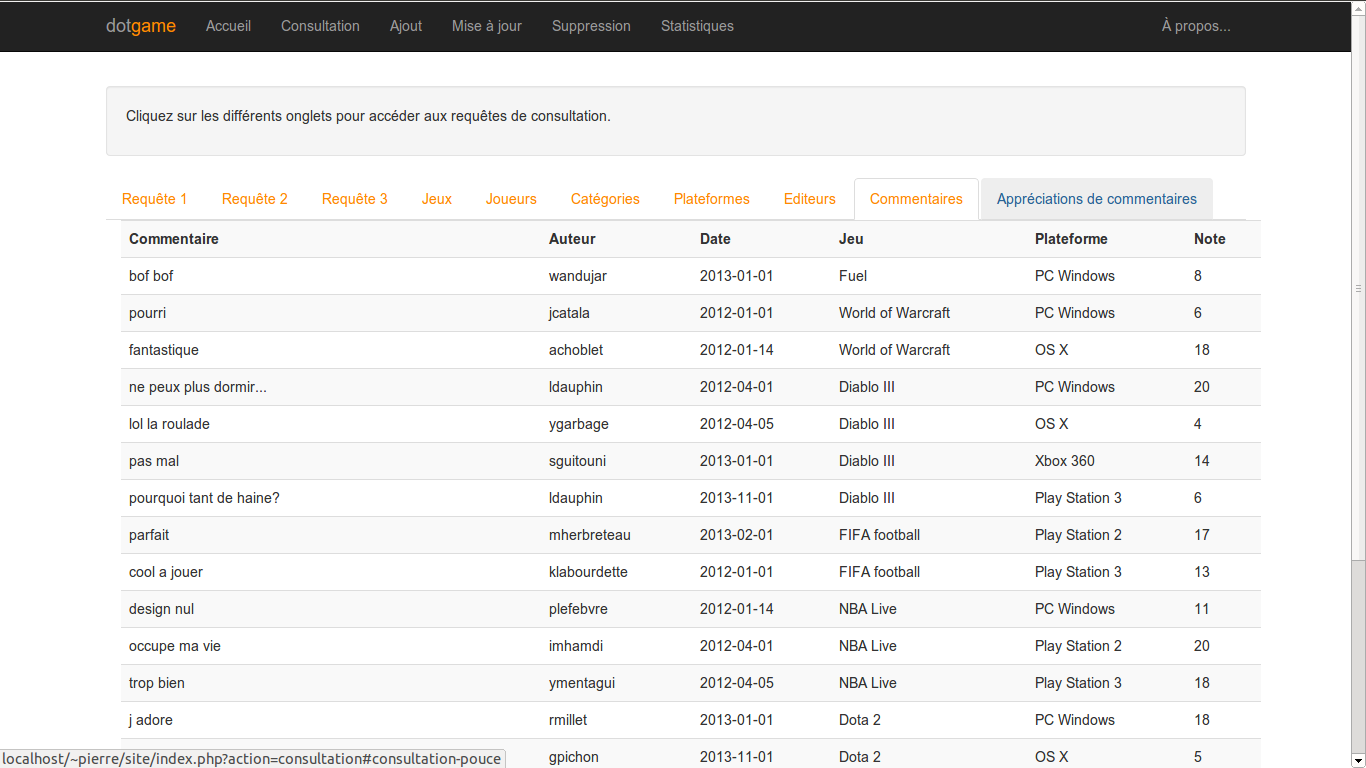
\includegraphics[width=0.8\textwidth]{capture1.png}
\end{center}
\caption{Vue de l'interface pour les consultations}
\label{fig:inter_consultation}
\end{figure}


\begin{figure}[!h]
\begin{center}
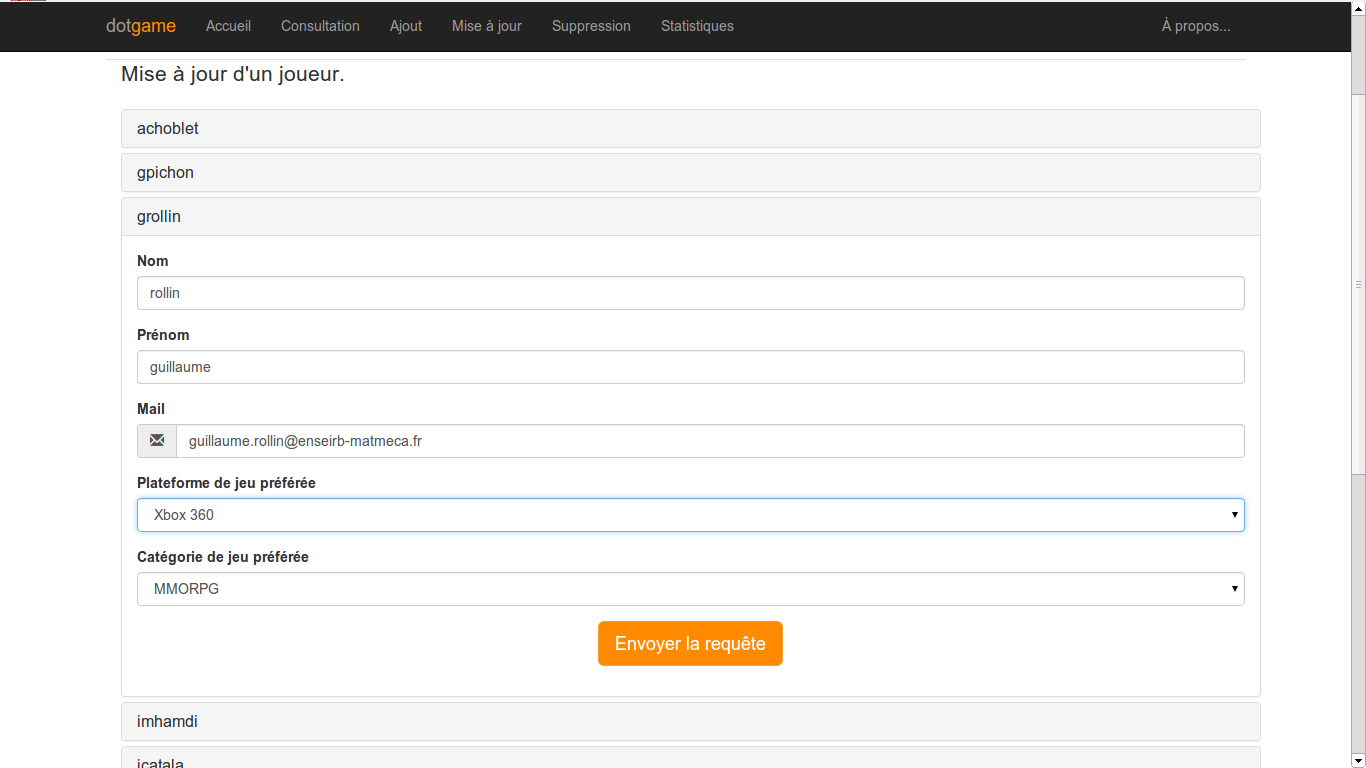
\includegraphics[width=0.8\textwidth]{capture2.png}
\end{center}
\caption{Vue de l'interface pour la mise � jour d'un joueur}
\label{fig:inter_maj}
\end{figure}


\subsection{Probl�mes - limites aux contraintes initialement fix�es}
